\begin{frame}[fragile]
\frametitle{Structure: Sections and Chapters}
    \LaTeX{} supports the creation of a dynamic logical document structure and enables customization of sectioning and numbering. \pause
\begin{exampleblock}{}
    \begin{minted}{latex}
    \section{Introduction}
    This is the introduction section. 
    \section{Second Section}
    This is the second section
    \end{minted}
\end{exampleblock} 
\begin{center}
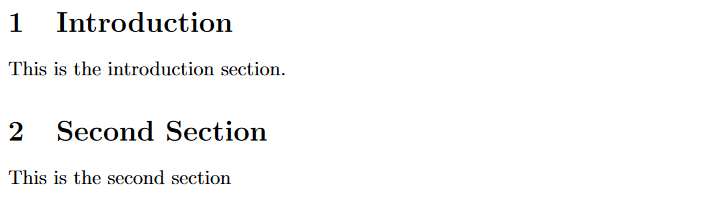
\includegraphics[width=0.8\linewidth]{img/sections_latex.png}
\end{center} \pause
\small For unnumbered sections, add an asterisk; that is, use \verb|\section*{}| instead of \verb|\section{}| and similarly for other sections.
\end{frame}


\begin{frame}[fragile]
\frametitle{Structure: Document Sectioning}
There are up to 7 levels of depth for defining sections depending on the document class. \pause
\begin{exampleblock}{}
    \begin{columns}
        \column{0.1\textwidth}
        -1 \\
        0 \\
        1 \\
        2 \\
        3 \\
        4 \\
        5 \\
        \column{0.7\textwidth}
        \verb|\part{part name}| \\
        \verb|\chapter{chapter name}| \\
        \verb|\section{section name}| \\
        \verb|\subsection{subsection name}| \\
        \verb|\subsubsection{subsubsection name}| \\
        \verb|\paragraph{paragraph name}| \\
        \verb|\subparagraph{subparagraph name}| \\
    \end{columns}
\end{exampleblock} \pause
In most cases, \verb|\section| is the top-level document command. For longer reports or books, \verb|\chapter| or \verb|\part| would be used instead.
\end{frame}


\begin{frame}[fragile]
\frametitle{Structure: The Table of Contents}
The table of contents is easily created with the \keytt{tableofcontents} command. \pause
\begin{exampleblock}{}
    \small
    \begin{minted}{latex}
    \tableofcontents
    \end{minted}
\end{exampleblock} \pause
Sections, subsections, and chapters ARE created in the table of contents; other document levels are NOT. \\[\baselineskip] \pause
Unnumbered sections can be manually added to the table of contents with \verb|\addcontentsline| immediately before the section declaration. \pause
\begin{exampleblock}{}
    \small
    \begin{minted}{latex}
    \addcontentsline{toc}{section}{Unnumbered Section}
    \section*{Unnumbered Section}
    \end{minted}
\end{exampleblock}
\end{frame}


\begin{frame}[fragile]
\frametitle{Structure: The Table of Contents}
The default title for the table of contents is ``Contents," but this is easily changed. \pause
\begin{exampleblock}{}
    \small
    \begin{minted}{latex}
    \renewcommand*\contentsname{Summary}
    \tableofcontents
    \end{minted}
\end{exampleblock} 
\vspace{0.2cm}
This will replace the default name ``Contents" with the new name ``Summary."
\end{frame}


\begin{frame}[fragile]
\frametitle{Structure: Page Numbering}
Page numbers are defined by their \keyw{style} and \keyw{location}. \pause
\begin{itemize}
    \item[$\bullet$] The \keyw{style} is changed with the \verb|\pagenumbering| command. \pause
    \item[$\bullet$] The \keyw{location} and format are changed with the \texttt{fancyhdr} package. \pause
\end{itemize}
\begin{block}{Page Number Styles}
\begin{minted}{latex}
\pagenumbering{⟨style⟩}
\end{minted}
Where \textit{style} is one of the following:
\begin{itemize} \small
    \item \texttt{arabic} (1, 2, 3, ...)
    \item \texttt{alph} (a, b, c, ...)
    \item \texttt{Alph} (A, B, C, ...)
    \item \texttt{roman} (i, ii, iii, ...)
    \item \texttt{Roman} (I, II, III, ...)
\end{itemize}
\end{block}
\end{frame}


\begin{frame}[fragile]
\frametitle{Structure: Page Numbering}
Internally, \LaTeX{} uses a \keyw{counter} to increment and keep track of the current page number. \pause
\begin{block}{Definition: Counter}
    A \emph{counter} is the name of a \LaTeX{} variable used to store an integer number. \LaTeX{} uses counters to internally track numbers of pages, figures, tables, equations, lists, etc. \\
    Internal counters can be manually changed or reset. New counters can be defined by the user.
\end{block} \pause 
The \LaTeX{} page counter variable is called \emph{\keytt{page}}.
\end{frame}


\begin{frame}[fragile]
\frametitle{Structure: Page Numbering}   
\small Counters controlling page numbering can be manually reset with the \keytt{pagenumbering} command at any point in the document. 
\begin{exampleblock}{} 
    \small
    \begin{minted}{latex}
    \pagenumbering{ style }
    \end{minted}
\end{exampleblock} \pause
\small Page number counters can be set to a specific value (\texttt{intval}) with the \keytt{setcounter} command.
\begin{exampleblock}{}
    \small
    \begin{minted}{latex}
    \setcounter{⟨countvar⟩}{⟨intval⟩}
    \end{minted}
\end{exampleblock} \pause
\small To add an amount (\texttt{increment}) to the counter variable (\texttt{countvar}), use the \keytt{addtocounter} command.
\begin{exampleblock}{}
    \small
    \begin{minted}{latex}
    \addtocounter{⟨countvar⟩}{⟨increment⟩}
    \end{minted}
\end{exampleblock} \pause
\small To add 1 to the count variable (\texttt{page}), use the \keytt{stepcounter} command.
\begin{exampleblock}{}
    \small
    \begin{minted}{latex}
    \stepcounter{ countvar }
    \end{minted}
\end{exampleblock} 
\end{frame}


\begin{frame}[fragile]
\frametitle{Structure: Multiple Columns}
\begin{itemize}
    \item[$\bullet$] For simple, two-column documents: pass the parameter \verb|twocolumn| to the initial \verb|documentclass| statement. \pause
    \item[$\bullet$] For more than two columns (or for more flexibility in column layout), use the \verb|multicol| package. \pause
    \item Specify number of columns in the \verb|\begin{multicols}{number of columns}| statement. \pause
    \item Column separation is handled with \verb|\columnsep|. \pause
\end{itemize}
\begin{exampleblock}{}
    \small
    \begin{minted}{latex}
    \usepackage{multicol}
    \setlength{\columnsep}{1cm}
    \end{minted}
\end{exampleblock}
\begin{exampleblock}{}
    \small
    \begin{minted}{latex}
    \begin{multicols}{2}
    Tomorrow, and tomorrow, and tomorrow,
    Creeps in this petty pace from day to day...
    \end{multicols}
    \end{minted}
\end{exampleblock}
\end{frame}


\begin{frame}[fragile]
\frametitle{Structure: Cross-References}
    \begin{wrapfigure}{r}{0.6\textwidth}
       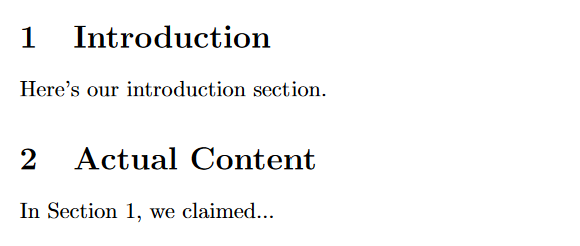
\includegraphics[width=0.58\textwidth]{img/crossrefexample.png}
   \end{wrapfigure}
   \LaTeX{} enables the cross-referencing of numbered items like equations, sections, chapters, figures, and tables internally within a document. \\
   For example, the command \verb|\label{ }| is used to set a label for an item like a section and the command \verb|\ref{ }| is used to reference it by number elsewhere in the document. 
   \small
   \begin{exampleblock}{}
    \begin{minted}{latex}
    \section{Introduction} \label{sec:intro}
    Here's our introduction section. 
    \section{Actual Content} 
    In Section~\ref{sec:intro}, we claimed...
    \end{minted}
   \end{exampleblock}
\end{frame}


% \begin{frame}[fragile]
% \frametitle{Structure: Cross-References}

% \end{frame}


\begin{frame}[fragile]
\frametitle{Structure: Cross-References with Hyperlinks}
To create hyperlinked references, load the \keytt{hyperref} package (optional \keytt{hidelinks} option avoids colored box around hyperlinks):
\begin{exampleblock}{}
\small
\begin{minted}{latex}
\usepackage{hyperref}  
\usepackage[hidelinks]{hyperref}
\end{minted}
\end{exampleblock} \pause
To manually set up link appearance:
\begin{exampleblock}{}
\small
\begin{minted}{latex}
\hypersetup{ ... }     
\end{minted}
\small
\keytt{colorlinks=true} \textit{Links color (default is red)} \\
\keytt{linkcolor=blue} \textit{Internal link color} \\
\keytt{filecolor=magenta} \textit{Local files link color} \\
\keytt{urlcolor=cyan} \textit{Website link color} 
\end{exampleblock} \pause
To keep urls in the same font/style as the rest of the document:
\begin{exampleblock}{}
\small
\begin{minted}{latex}
\urlstyle{same}
\end{minted}
\end{exampleblock}
\end{frame}


\begin{frame}[fragile]
\frametitle{Structure: Hyperlinks}
To link web addresses, use either the \keytt{url} package (displays the url text) or the \keytt{hyperref} package (displays hyperlinked alt text). \pause
\begin{exampleblock}{Example (Hyperlinks and URLs)}
\begin{minted}{latex}
For further reference, see 
\href{https://www.youtube.com/watch?v=dQw4w9WgXcQ}
{A Totally Normal Link} 
or go to the url: 
\url{https://www.youtube.com/watch?v=dQw4w9WgXcQ}
\end{minted}
\end{exampleblock}
\vspace{0.2cm}

\includegraphics[width=\linewidth]{img/hyperlink_ex.png}
\end{frame}



\begin{frame}[fragile]
\frametitle{Structure: More fun structure things!}
\begin{itemize}[$\bullet$]
    \item The \texttt{titlesec} package can be used to customize chapters, sections, subsections etc. \pause
    \item Document class: \texttt{report}. \pause
    \item Document class:  \texttt{book}. \pause
    \item Unbalanced columns. \pause
    \item Floating elements in columns. \pause
    \item Vertical rulers between columns. 
\end{itemize}
\end{frame}


% \begin{frame}[fragile]
% \frametitle{Structures: Summary}

% \end{frame}



% \begin{frame}[fragile]
% \frametitle{Structure: Summary}
    
% \end{frame}
